\documentclass[12pt]{article}

% Preamble area where you can include packages
\usepackage[utf8]{inputenc} % Encoding
\usepackage[T1]{fontenc}    % Font encoding
\usepackage{amsmath}        % Advanced math typesetting
\usepackage{amsfonts}       % Mathematics fonts
\usepackage{amssymb}        % Mathematics symbols
\usepackage{graphicx}       % Include images
\usepackage{hyperref}       % For hyperlinks in the document
\usepackage{lipsum}         % Generates dummy text

% Metadata
\title{CA Lab1 Report}
\author{Yu-Xiang Luo}
\date{\today} % You can set a specific date with \date{YYYY-MM-DD}

\begin{document}

\maketitle % Creates the title, author, and date

\section*{\texttt{ALU.v}}
\begin{itemize}
	\item In \texttt{ALU.v}, we follow the table below to recognize the \texttt{ALUCtrl}, and do the right thing.
	\item In this module, the input would be two data and a control, and the output is the calculation.
\end{itemize}

{
	\centering
	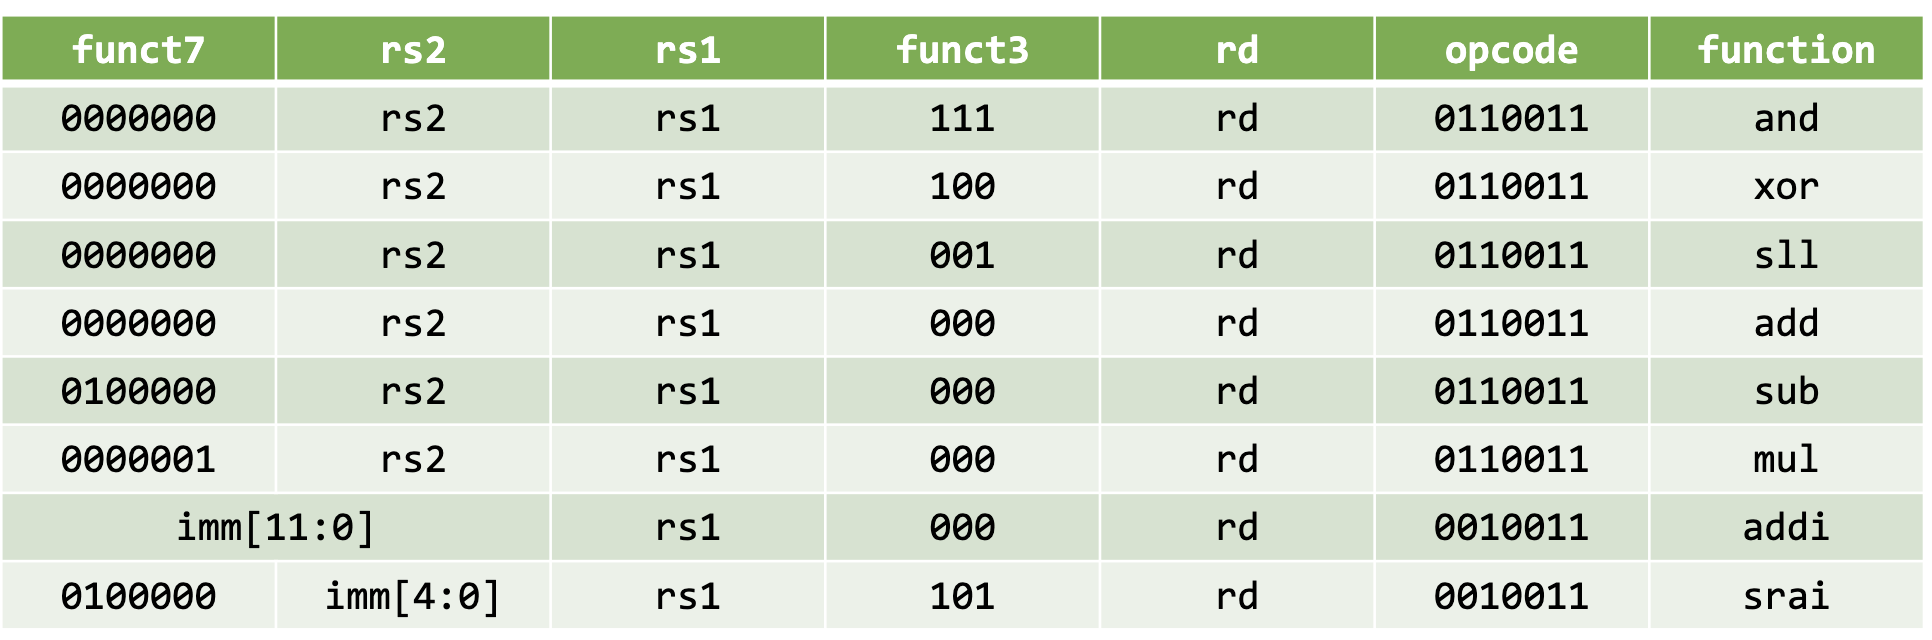
\includegraphics[width=\textwidth]{./img/ALU_table.png}
}

\newpage
\section*{\texttt{ALU\_Control.v}}
\begin{itemize}
	\item In \texttt{ALU\_Control.v}, I did some modification, I replace the \texttt{ALUCtrl} to binary order, so if you take a look to the code, the ALU Control is not defined in riscv-style.
		\begin{table}[h!]
			\centering
			\begin{tabular}{|c|c|}
				\hline
				Operation & ALU Control \\ \hline
				AND  & b000  \\ \hline
				XOR  & b001  \\ \hline
				SLL  & b010  \\ \hline
				ADD  & b011  \\ \hline
				SUB  & b100  \\ \hline
				MUL  & b101  \\ \hline
				ADDI & b110 \\ \hline
				SRAI & b111 \\ \hline
			\end{tabular}
		\end{table}
\end{itemize}

\section*{\texttt{Adder.v}}
\begin{itemize}
	\item This is just an adder.
\end{itemize}

\section*{\texttt{CPU.v}}
\begin{itemize}
	\item I think it's the most tricky part. To do this right, you have to connect the wire correctly, and assign them is also a trivial task, you have to make sure it's the same as the graph in slides.
\end{itemize}
{
	\centering
	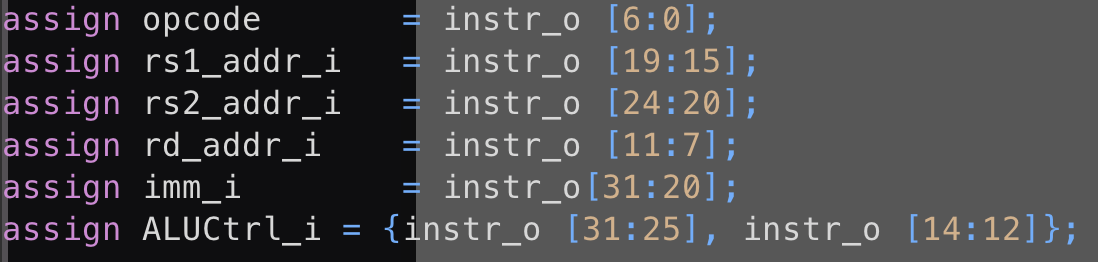
\includegraphics[width=\textwidth]{./img/CPU_code.png}
}

\section*{\texttt{Control.v \& MUX32.v}}
\begin{itemize}
	\item Parse the Opcode correctly, it's straightforward as the code shows, no explanation.
\end{itemize}

\section*{\texttt{Sign\_Extend.v}}
\begin{itemize}
	\item To do the \textbf{sign} extend, I make the \textbf{MSB} extend for 20 times. You can view code for details.
\end{itemize}

\end{document}

